% --------------------------------------------------------------------

\section{Johdanto}

\begin{comment}
\textbf{DISCLAIMER V1:} Huonoa, muistiinpanonomaista tekstiä. Tullaan parantamaan.
\textbf{DISCLAIMER V2:} Perusasiat alkaa olla selitetty, joskin teksti on hiomatonta
ja mitä luultavimmin täynnä kirjoitus- ja lyöntivirheitä.
\end{comment}

Nykyaikainen videodata tallennetaan digitaaliseen muotoon. Videodatan
käsittelyä digitaalisille tallennuslaitteille ja siirtokanaville sopivaan
muotoon ja uudelleen katseltavaan muotoon kutsutaan videokoodaukseksi.
Koodaaminen on tärkeää kaikenlaisen median, kuten äänen, kuvan ja videon,
digitaaliselle tallentamiselle. Videodatan erikoisominaisuus on se, että
se yhdistelee erilaisia medioita. Tämän seurauksena videodata vaatii suuren
määrän tallennustilaa ja siirtokapasiteettia, mikä tekee videon koodaamisesta
tärkeämpää. Samalla videodatan monialainen luonne lisää haasteita sen
kompaktiin esittämiseen. Olemassa olevia videokoodausmenetelmiä määräävät
standardi. (\citealt{h264})

Videodatan laadun kasvu ja tiedon langattoman siirtämisen yleistyminen pakottaa
kehittämään uusia, tehokkaampia videokoodausmenetelmiä. Ollaan kuitenkin tultu
siihen pisteeseen, että vain tehokkaimmat yksiprosessorijärjestelmät pystyvät
koodaamaan korkealaatuista videodataa. Kustannustehokkaan ja riittävän
laskentatehon saavuttamiseksi tarvitaan tulevaisuudessa muita ratkaisuja, kuin
ainainen yksittäisen prosessorin kellotaajuuden kasvatus. Rinnakkaislaskenta
mahdollistaa halvemman ja paljon tehokkaamman ratkaisun laskentatehon
kasvattamiseen. (\citealt{xu}, \citealt{chi}) Rinnakkaislaskenta on siitäkin
luonnollinen ratkaisu, että moniydinprosessorijärjestelmät yleistyvät
vauhdilla, minkä lisäksi lähes jokaisessa nykyaikaisessa tietokoneessa on
grafiikkaprosessori, joka on luonteeltaan hyvin rinnakkainen (\citealt{choi}).

Sopivuudestaan huolimatta rinnakkaisohjelmointi ei kuitenkaan ole helppo
ratkaisu laskentatehon lisäämiseksi. Jotta rinnakkaisista järjestelmistä
saataisiin laskennallista hyötyä, täytyy laskenta järjestää huolellisesti.
Eri laskentayksiköiden välinen kommunikaatio, laskennan synkronointi ja
oikeellisuus ovat rinnakkaisohjelmoinnin suuria haasteita.
Rinnakkaisohjelmoinnin ongelma on myös se, että pitkään sillä saavutetut hyödyt
olivat pieniä verrattuna normaaliin laskentaan sen vaikeuksista johtuen. (\citealt{intro})
Toisaalta Mooren lain mukainen prosessoreiden tehon kasvu on tarkoittanut sitä,
että horisontissa on aina ollut tehokkaampia prosessoreita (\citealt{moore}). Nyt kuitenkin
alettu saavuttaa raja, jossa kaikkia yksittäiselle sirulle asetettuja
transistoreita ei voida käyttää esimerkiksi jäähdytyksen riittämättömyyden
johdosta. Rinnakkaiset ratkaisut ovat tulevaisuudessa välttämättömiä.

Rinnakkaisuuden omien ongelmien lisäksi videokoodaus tuo rinnakkaislaskentaan
omat haasteensa. Videodata on luonteeltaan moninaista ja sillä on runsaasti
sisäisiä riippuvuuksia. Lähes kaikki nykyiset videokoodausmenetelmät
hyödyntävät näitä riippuvuuksia koodausta nopeuttaakseen ja tallennustilaa
säästääkseen, mutta rinnakkaislaskennan kannalta nämä riippuvuudet vähentävät
rinnakkaistamisen mahdollistamista. Nykyisiä standardeja ei ole suunniteltu
rinnakkaisuutta silmällä pitäen. (\citealt{pieters}, \citealt{xu})

Videokoodauksen rinnakkaistaminen vaatii edellisissä kappaleissa esitettyjen
ongelmien ratkaisua, eivätkä ongelmat määrästään huolimatta ole mahdottomia.
Datan riippuvuuksia voidaan rikkoa, laskenta järjestää tehokkaaksi ja uusia
standardeita kirjoittaa. Rinnakkaislaskennalla on tuotu onnistuneesti lisätehoa
jo olemassa oleviin menetelmiin ja tulevien standardien suunnittelussa
rinnakkaisuus on jo otettu huomioon. (\citealt{li}, \citealt{chi})
Rinnakkaisohjelmointi tulee yleistymään kaikilla tietotekniikan
sovellusalueilla ja rinnakkaisohjelmointityökalut kehittymään. Vaikeuksista
huolimatta rinnakkaislaskenta on myös videokoodauksen tulevaisuutta.

Tämä työ keskittyy esittelemään ratkaisuja videokoodauksen rinnakkaistamiseen.
Lisäksi esitellään videokoodauksen ja rinnakkaislaskennan perusasioita, jotta
rinnakkaisen videokoodauksen hyödyt, tarpeellisuus ja haasteet tulisivat
esille. Aluksi esitellään digitaalisen liikkuvan kuvan peruskäsitteitä,
rinnakkaislaskennan historiaa ja joitakin näitä tukevia tieteenaloja. Tämän
jälkeen esitellään videokoodaus ja rinnakkaislaskenta. Lopulta esitellään
varsinaisia ratkaisuja rinnakkaiseen videokoodaukseen ja tehdään yhteenveto
tutkimuksen sisällöstä.

\newpage

\section{Digitaalinen liikkuva kuva ja rinnakkaislaskennan perusteet}

Tässä luvussa käsitellään digitaalista videota, rinnakkaislaskennan historiaa
sekä kahta liikkuvaan kuvaan ja rinnakkaislaskentaan liittyvää käsitettä,
havaitsemista ja rinnakkaislaskennan oikeellisuutta. Luvun tavoitteena on
toimia johdantona työn aiheisiin eikä niissä syvennytä mainittuihin teemoihin
kovin tarkasti.

\subsection{Digitaalinen video ja sen koodaus}

Ennen kuin puhutaan digitaalisesta videosta, täytyy ymmärtää liikkuvan kuvan
perusteita. Ensimmäisistä liikkuvan kuvan sovelluksista 1800-luvun lopulta
alkaen elävä kuva on perustunut samaan ajatukseen, eli peräkkäisten kuvien
nopeaan peräkkäiseen näyttämiseen liikkuvan kuvan vaikutelman aikaansaamiseksi.
Eräs ensimmäisistä ja pisimpään selvinneistä tallennusformaateista oli filmi,
jolle valotettiin peräkkäisiä valokuvia ja tulosta esitettiin projektorilla.
Vuosien saatossa tallennusmenetelmät ovat kehittyneet ja siirtomenetelmät
kehittyneet ensin analogisiksi radiosignaalien esimerkin innoittamana ja
myöhemmin digitaalisiksi digitaalisen vallankumouksen myötä. (\citealt{mitra})
Kuvaamisen ja tallentamisen periaatteet ovat kuitenkin samat läpi
historian.

Viimeisen viidentoista vuoden aikana suurin osa videodatasta on muuttunut
analogisesta digitaaliseksi. VHS-kaseteista ja analogisista TV-lähetyksistä
on siirrytty Blu-Ray -tekniikoihin, kännykkäkameroihin
teräväpiirtotelevisioihin. Tekniikan kehitys ei näy ainoastaan tallennusmedioissa,
sillä niin ikään tiedonsiirto on kehittynyt ja muuttunut monin paikoin
langattomaksi.(\citealt{h264})
Digitaalisen videodatan määrä on myös valtavassa kasvussa (\citealt{cisco}, \citealt{youtube}).
Raaka videodata vaatii suuret määrät tallennustilaa eikä sen siirtäminen
langattomasti ole mahdollista - tarvitaan siis teknologia, jolla videodataa pakataan ja puretaan
(enkoodataan ja dekoodataan). Tätä pakkaamisen ja purkamisen prosessia
kutsutaan videokoodaukseksi. Pakkaamisen ja purkamisen lisäksi videokoodaus kattaa
myös signaalin reaaliaikaisesta kääntämisestä (transkoodaus). Transkoodaus
tarkoittaa esimerkiksi enkoodatun datan kääntämistä toiseen koodausstandardiin (\citealt{mpeg_app}).
Seuraavissa alaluvuissa käsitellään videokoodausmenetelmien perusteita. Tästä lähin näihin viitataan termein
enkoodaus, dekoodaus ja transkoodaus. Toinen kirjallisuudessa esiintyvä ja
tärkeä termi on CODEC (COder DECOder pair), joka viittaa videokoodausta suorittavaan
ohjelmistoon tai laitteeseen(\citealt{h264}). Suomeksi CODEC taipuu koodekiksi.

Videokoodausstandardeja on useita, mainittakoon tässä H.264, MPEG-4 ja DICOM,
joista kaksi ensimmäistä ovat kuluttajakäyttöön suunniteltuja standardeja
ja viimeinen lääketieteelliseen kuvantamiseen suunniteltu.

\subsection{Rinnakkaislaskennan perusteita}

Rinnakkaislaskennan (parallel computing) tavoite on parantaa laskennan
suorituskykyä. Käsitteellisesti rinnakkaislaskentaa ei kannata sekoittaa
samanaikaiseen laskentaan (concurrent computing). Akateemisessa mielessä
jälkimmäinen keskittyy rinnakkaisen laskennan oikeellisuuteen, kun taas
ensimmäinen keskittyy saamaan hajautetusta ja rinnakkaisesta laskennasta
näkyviä hyötyjä laskentatehoon. (\citealt{intro}, \citealt{ari}) Tämä työ keskittyy
rinnakkaisella laskennalla saavutettuihin hyötyihin videokoodauksen saralla,
mutta myöhemmin tässä luvussa esitellään lyhyesti rinnakkaislaskennan
oikeellisuuden tarkastelua.

Rinnakkaislaskennan nimi on suuntaa-antava. Suorituskykyä pyritään parantamaan
suorittamalla laskentaa mahdollisimman monella laskentayksiköllä samaan aikaan.
Ajatus on looginen - jos yhdeltä laskentayksiköltä kestää yhden aikayksikön
suorittaa jokin laskentatehtävä, niin sadan laskentayksikön suorittaminen
kestää sata aikayksikköä. Sadalta laskentayksiköltä taas menee samaan tehtävään
vain yksi aikayksikkö. Yksinkertaiseen perusidea monimutkaistuu kuitenkin
käytännössä valtavasti. Entä jos laskentatehtävät riippuvat muista
laskentatehtävistä? Miten laskentayksiköt kommunikoivat keskenään ja mihin
tieto tallennetaan? Nämä ongelmat saattavat tuntua pieniltä, mutta niiden
johdosta rinnakkaislaskenta on pysynyt kehityksen marginaalissa vuosikymmeniä.
(\citealt{intro}) Rinnakkaislaskennan tuoma laskentatehon hyöty ei myöskään ole
maailmaa mullistava, rinnakkaislaskenta ei esimerkiksi sovellu NP-täydellisten
ongelmien poistamiseen ratkaistavien ongelmien listalta. NP-ongelmien
ratkaisemiseksi tarvittaisiin ongelman kokoon nähden eksponentiaalinen määrä
laskentayksiköitä, eikä tämä ole käytännöllistä.

\subsection{Havaitseminen}

Video on visuaalinen media ja havaitseminen on sitä vahvasti tukeva
tutkimusala. Videokoodauksen kannalta havaitseminen on mielenkiintoista
videodatan subjektiivisen laadun takia. Subjektiivista laatua käsitellään
myöhemmin tässä työssä, mutta kerrottakoon tässä, että videodatan laatua
voidaan pakatessa menettää ilman, että ihmissilmät havaitsee laadun
heikkenemistä. Tätä tosiasiaa voidaan käyttää tiiviimmän pakkaamisen
aikaansaamiseksi. (\cite{h264})

Havainnoinnin tutkimustyökaluja ovat muun muassa silmien liikkeiden seuraus,
kyselytutkimukset ja aivojen kuvantaminen. Videodatan subjektiivista laatua
ja näin erästä videokoodauksen onnistumisen kriteeriä voidaan mitata
kyselytutkimuksella. Joitakin havaitsemistutkimuksen tuloksia on myös käytetty
videokoodausmenetelmien kehittämiseen. Eräs tutkimus on parantanut videodatan
subjektiivista laatua tutkimalla silmän liikkeitä ja parantanut yleisimpien
havainnoinnin kohteena olleiden alueiden tarkkuutta videossa
(\citealt{perception}). Toinen tutkimus on dekoodannut liikkuvia kohteita
videossa suuremmalla tarkkuudella, sillä ihmissilmä keskittyy luontaisesti
liikkeeseen (\citealt{lee}).

Huomattavaa on siis, että monista tieteenaloista on hyötyä videokoodaukselle.
Menetelmiä voi aina parantaa, mutta keskittymällä olennaisiin parannuksiin
päästään vähemmällä vaivalla.

\subsection{Rinnakkaislaskennan oikeellisuus}

Laskentatehon lisäyksen lisäksi rinnakkaisuus lisää virhelähteitä laskentaan.
Muistin käsittely, laskennan aikataulutus ja viestikanavien käyttö ovat
esimerkkejä virheläheistä, joita ei perinteisessä peräkkäisessä ohjelmoinnissa
esiinny. Rinnakkaisten järjestelmien oikeellisuuden tarkastelua vaikeuttaa se,
että virheitä on vaikea toistaa, sillä ne saattavat riippua hyvin tarkoista
ajoituksista ja sopivista suoritusjärjestyksistä ohjelman ajon aikana. Kaikki
ehdot eivät välttämättä kaikkien ajojen aikana toteudu ja virheitä on vaikea
löytää ja toistaa. Nämä seikat lisäävät ongelmia rinnakkaisohjelmien
toteutukseen kaiken muun mainitun lisäksi. (\citealt{ari})

Yrityksellä ja erehdyksellä virheiden etsiminen on kallista ja aikaa vievää,
joten parempia keinoja tarvitaan. Eräs analyyttinen ratkaisu
rinnakkaislaskennan oikeellisuuden tarkasteluun on mallintarkistus. Tässä
menetelmässä rinnakkainen ohjelma kuvataan mallina, joka täyttää jollekin
abstraktion tasolle asti ohjelmalle asetetut vaatimukset. Mallia voidaan
tutkia automaattisilla työkaluilla, jotka paljastavat mahdollisia
rinnakkaisuuden ongelmia, kuten muistin ylikirjoittamista, ei-toivottuja
kisatilanteita tai laskennan umpikujia (deadlock). (\citealt{ari})
Mallintarkastus on laskennallisesti erittäin vaativa tehtävä, mutta se saattaa
säästää järjestelmän myöhemmiltä, mahdollisesti hyvin kalliilta ja vaikeilta
ongelmilta.


\begin{comment}
-tähän lukuun:

	-videokuvasta palikka-asiaa

	-rinnakkaisohjelmoinnista palikka-asiaa

	-havaitsemisesta jotain palikka-asiaa

	-videokoodauksessa paljon standardeja

	-rinnakkaislaskentaa yritetty jo vuosikymmeniä saada toimimaan
\end{comment}

\newpage

\section{Videokoodaus}

Tässä luvussa käsitellään videokoodauksen perusteita. Luvun tavoite on
antaa riittävät taustatiedot videokoodausmenetelmistä, jotta myöhemmässä
vaiheessa tätä työtä voidaan esitellä rinnakkaisia
videokoodausmenetelmiä sekä antaa hyvä yleiskuva videokoodauksesta. Yleisen
käsittelyn lisäksi tekstissä on esitelty lyhyesti muutama mielenkiintoinen
tutkimus, jotka ratkovat joitakin videokoodauksen ongelmia.

\subsection{Videokoodauksen peruskäsitteet}

\subsubsection{Videokuvan esittäminen ja tallentaminen}

Havaitsemamme maailma on täynnä erilaisia kohteita, joilla on
erilaisia ominaisuuksia, kuten muoto, syvyys, tekstuuri, väri tai valotiheys.
ja joita videolle haluttaisiin tallentaa. Maailma on niin ikään jatkuva,
mitä esimerkiksi digitaalinen maailma ei ole. Jotta kameralla tai vastaavalla
laitteella voitaisiin tallentaa esitys maailmasta, täytyy havainnot käsitellä ja
tallentaa digitaaliseen maailmaan sopivaksi. Tässä luvussa käsitellään
erialisia keinoja tallentaa videodataa - otantoja, ennustamista, väriavaruuksia
ja näihin liittyviä matemaattisia tekniikoita ja käsitteitä.

Videodataa varten maailmasta täytyy kerätä näytteitä eri ajanhetkiltä. Otanta
tapahtuu kahdessa ulottuvuudessa, ajassa ja tilassa (temporal and spatial
sampling). Tyypillisesti tilaotokset ovat suorakaiteen muotoisia kuvia
maailmasta, kun ajallinen otanta koostuu peräkkäisistä tilaotoksista.
Tilaotokset koostuvat neliönmuotoisista kuvapisteistä eli pikseleistä, jotka
on järjestetty ruudukoksi. Tilaotoksia peräkkäin toistamalla saadaan aikaan
vaikutelma elävästä kuvasta. Tällainen data (käsittelemättömät aika- ja
tilanäytteet) tunnetaan myös raakadatana. (\citealt{h264}, \citealt{du})

Jokaisen tilanäytteen kuvapisteeseen tallennetaan pisteeseen liittyvät
tiedot. Yksinkertaisinta kuvaa eli mustavalkokuvaa varten riittää esimerkiksi
tallentaa vain yksi arvo kuvapisteestä (kirkkaus tai valotiheys), mutta
värikuvassa täytyy tallentaa jokaisessa pisteessä esiintyvien värien määrä.
Väriavaruudeksi kutsutaan menetelmää, joka on valittu kuvapisteiden kirkkauden,
valotiheyden ja värin kuvaamiseksi. Värikuvan tallentamisessa suosittu tapa on
RGB-väriavaruus. Tässä menetelmässä jokaisella kuvapisteellä on
kolme parametria: punaisen, vihreän ja sinisen värin määrä. Edistyneemmät
väriavaruudet hyödyntävät ihmisaivojen suurempaa herkkyyttä valotiheydelle
kuin väreille (RGB-väriavaruudessa valotiheys ja väri ovat samanarvoisia
tietoja). (\citealt{h264}, \citealt{du}) Huomattavaa on, että väriavaruudet ovat matemaattisia
malleja havaitusta maailmasta. Niille on paljon erilaisia implementaatioita,
joihin ei tämän työn puitteissa syvennytä tarkemmin.

Avaruudellisia näytteitä voidaan ottaa joko peräkkäin (progressive) tai
lomittain (interlacing). Peräkkäisessä otannassa jokaisella ajanhetkellä
otetaan otos, johon tallennetaan käytössä olevan standardin mukainen
määrä kuvapisteitä. Otosta kutsutaan ruuduksi (frame). Lomittaisessa
otannassa taas jokaisella ajanhetkellä tallennetaan puolet standardin
määräämistä kuvapisteistä vaakasuunnassa joka toinen rivi siten, että
peräkkäisillä ajanhetkillä tallennetaan lomittaiset rivit. Otosta kutsutaan
kentäksi (field). Erotuksena näillä metodeilla on siinä, että lomittaisella
otannalla syntyy pehmeämmin liikkuvaa kuvaa kuin peräkkäisellä otosten määrän
ollessa sama. Lomittamalla jokaiseen otokseen tallennetaan myös vähemmän tietoa.
(\citealt{h264}, \citealt{du})

\subsubsection{Videodatan muut osat ja synkronointi}

Videodata ei koostu ainoastaan varsinaisesta videokuvasta, vaan kuvan lisäksi
tallennusvaiheessa tallennetaan ääntä. Ääniraita enkoodataan kuvadatan tavoin
halutulla menetelmällä ja tallennetaan kuvadatan oheen (\citealt{mpeg_app}). Tässä
työssä ei syvennytä tarkemmin äänen koodaamiseen, mutta perusperiaatteet
pakkausmenetelmissä ovat samankaltaiset. Kuvan ja äänen lisäksi videokoodauksen
eri vaiheissa dataan voidaan lisätä haluttuja ominaisuuksia. Suomessa tutuin
lisä on tekstitys, joka muiden lisäominaisuuksien tavoin usein tallennetaan
varsinaisesta videodatasta erillään. On myös mahdollista tallentaa tieto
lisäominaisuuksista koodattuun videodataan - tätä kutsutaan tiedon
piilotukseksi ja sillä saavutetaan pieniä etuja pakkauksen koon suhteen
pientä videon laadun menetystä vastaan. (\citealt{hiding}) Tällöin
lisäominaisuuksien synkronointi ei ole tarpeen.

Videodatan osien ollessa erillisiä kuitenkin tarvitaan keino tahdistaa data eri
lähteistä hyvän katselukokemuksen takaamiseksi. Perusmenetelmiä on kolme.
Ensimmäinen on aikaleimatahdistus (Time-Stamps Synchronization), jossa eri
lähteisiin lisätään aikaleimoja. Aikaleimojen perusteella osataan eri lähteistä
tuleva data näyttää käyttäjälle samanaikaisesti. Toinen keino on
tahdistusmerkki (Synchronization Marker), joka käytännössä tarkoittaa eri datalähteiden välistä
kommunikaatiota, käytännössä merkin lähettämistä ja vastaanottamista, tahdistuksen
saavuttamiseksi. Kolmas on 	limitystahdistus (Multiplex Synchronization), jossa
limitetään eri datalähteet yhdeksi lähteeksi hyödyntäen näin niiden
luonnollista järjestystä tahdistuksen saavuttamiseksi. Nauhoittaessahan kuva ja
ääni ovat tahdistettu. Perusmenetelmien lisäksi on tutkittu erilaisia metodeita
sulauttaa lisäominaisuuksien lisäksi myös audio varsinaiseen videodataan.
Tällöin enkoodausvaiheessa kuvadataan lisätään äänidataa. Tehdyssä
tutkimuksessa videon tai kuvan laadun heikkeneminen ei ollut ihmissilmällä
havaittavissa. (\citealt{sync}, \citealt{mujal})

\subsubsection{Pakkaus}

Kaikenlaisen median pakkausmetodit voidaan jakaa häviöttömiin
ja häviöllisiin pakkausmetodeihin (lossy, lossless). Häviöttömissä metodeissa pakatusta datasta
pystytään purkuvaiheessa palauttamaan täydellinen versio alkuperäisestä
datasta, häviöllisessä pakkauksessa purettu versio on approksimaatio
alkuperäisestä. On olemassa häviöttömiä videokoodausmenetelmiä, mutta
pakkaussuhde jää liian alhaiseksi käytännön sovelluksiin. Häviölliset
pakkausmenetelmät keskittyvät poistamaan datasta subjektiivista redundanssia,
eli sellaisia yksityiskohtia, jota havainnoija ei kykene havaitsemaan. Näin
saavutetaan huomattavasti tehokkaampia videokoodausmenetelmiä. (\citealt{h264}, \citealt{du})
Toisaalta esimerkiksi lääketieteelliset sovellukset tai konenäkösovellukset
vaativat korkealaatuista kuvaa, jolloin häviötön pakkaaminen on ainoa
vaihtoehto (\citealt{xu}).

Suurin osa videokoodausmenetelmistä hyödyntää videodatan vahvaa
avaruudellista ja ajallista redundanssia. Käytännössä peräkkäisissä
ruuduissa on suurella todennäköisyydellä lähes samat kuvapisteet (ajallinen) ja
yhdessä ruudussa lähekkäiset kuvapisteet muistuttavat toisiaan suurella
todennäköisyydellä (avaruudellinen). Monien koodekkien ensimmäinen askel videon koodaamiseen
on ennustaminen - jollakin määrällä edellisiä ajallisia näytteitä voidaan
melko suurella todennäköisyydellä ennustaa, mitä tässä näytteessä tulee
olemaan. Samaan tapaan saman näytteen sisällä jo käsiteltyjen kuvapisteiden
perusteella ennustetaan tulevien kuvapisteiden laatua. Ennustuksilla voidaan
vähentää tallennettavan datan määrää, kun purkuvaiheessa näytteitä pystytään
uudelleenrakentamaan edellisten näytteiden perusteella. Läheisesti
ennustamiseen liittyvä käsite on liikekompensaatio (motion compensation).
Käytännössä liikekompensaatio on ennustamisen apukeino. Esimerkiksi kameran
kääntyessä ei verrata peräkkäisissä näytteissä samoilla koordinaateilla
olevia kuvapisteitä vaan myös sopivalla tavalla lähialueilta valittuja
pisteitä. (\citealt{h264}, \citealt{du})

\subsection{Videodatan riippuvuudet}

Videodata on luonteeltaan monijakoista sen sisältäessä niin liikkuvaa kuvaa,
ääntä kuin mahdollisia lisäominaisuuksia. Näiden sekä
enkoodauksen aikaisen ennustamisen johdosta koodatulla videodatalla on vahvoja
riippuvuussuhteita. Riippuvuuksia on kahdentyyppisiä. Ajallinen riippuvuus
tarkoittaa tässä yhteydessä sitä, että onnistunut videodatan
toistaminen on riippuvainen kaikista videodatan osien samanaikaisesta
toistamisesta. Datariippuvuutta syntyy ruutujen ja kenttien
sisällä esimerkiksi ennustettaessa uuden kuvapisteen arvoa edellisten
kuvapisteiden perusteella tai uusia näytteitä ennustettaessa  vanhojen
perusteella. (\citealt{mujal})

Riippuvuudet vaikeuttavat videokoodausprosessia ja lisäävät siihen ylimääräisiä
vaiheita ja monimutkaisuutta, kuten synkronointi (pelkän äänen tai kuvan koodaaminen on paljon helpompaa).
Seuraavassa aliluvussa käsiteltävä diskreetti kosinimuunnos ja muut koodaukseen
liittyvät operaatiot eivät ole itsessään kovin vaativia, mutta koodekit ovat
kuitenkin varsin suuria ohjelmistoja kaiken laskentaa tehostavien lisäysten
johdosta. Esimerkiksi x264-ohjelmisto, joka on avoimen lähdekoodin toteutus
suositusta H 264 -standardista (\citealt{h264}), on n. 100 000 riviä koodia (\citealt{x264}).

Erityisesti riippuvuudet vaikeuttavat erilaisten koodausalgoritmien rinnakkaistamista -
rinnakkaislaskennassa yhden laskentayksikön laskemat tulokset ovat toisille
yksiköille käytännössä saavuttamattomissa. Rinnakkaisuuden ja riippuvuuksien
ongelmia käsitellään myöhemmin riinnakaislaskentaa sekä rinnakkaista
videokoodausta käsittelevissä luvuissa.
On kuitenkin myös esitetty runsaasti keinoja, joilla riippuvuuksista päästään
eroon. Ennustaminen toimii hyvin peräkkäisissä koodausmenetelmissä, mutta
videolaadun kasvaessa peräkkäiset ratkaisut alkavat olla liian tehottomia (\citealt{choi}, \citealt{xu}).
Luoviakin ratkaisuja on tehty - \citealt{lee} ehdottaa menetelmää, jossa videon
äänilähteet piirretään suuremmalla tarkkuudella, koska ihmisten on luonteva
keskittää huomionsa äänilähteisiin. Tämä parantaa videon subjektiivista laatua,
johon palataan myöhemmässä aliluvussa. Mainitut lähteet (\citealt{mujal},
\citealt{sync}) esittelevät keinoja helpottaa videodatan synkronointia ja vähentää
tallennustilan tarvetta subjektiivisen laadun pysyessä käytännössä samana.

\subsection{Diskreetti kosinimuunnos}

Ennen tallentamista tai siirtämistä videodataa useimmiten käsitellään vielä
jollain tavalla ennustusten lisäksi. Tavoitteena on vähentää tallentamiseen
tarvittavaa muistia ja helpottaa aikanaan tapahtuvaa dekoodausta. Tekniikoita
on monia, mutta esitellään tässä yleisin, eli diskreetti kosinimuunnos
(Discrete Cosine Transformation, DCT). 

DCT on Fourier-muunnoksen kaltainen muunnos, joka operoi $N \times N$
kokoisilla blokeilla avaruudellisissa näytteissä. Muunnos tuottaa niin
ikään $N \times N$ kokoisen blokin, mutta kuvapisteiden arvojen sijaan
uuden blokin arvot ovat kosinimuunnoksen peruslohkojen suhteellisia
voimakkuuksia koodattavassa olevassa lohkoissa. Kuvassa \ref{fig:dct} on esitetty
$8  \times 8$ -lohkon DCT:n peruslohkot. (\citealt{h264})

\begin{figure}[ht]
	\centering
	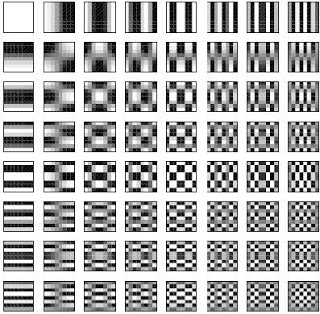
\includegraphics[width=0.5\textwidth]{dct.jpg}
	\caption{$8 \times 8$ DCT:n peruslohkot}
	\label{fig:dct}
\end{figure}

DCT:n hyöty ei ole ilmeinen, sillä muunnos tapahtuu $N \times N$ -lohkosta
$N \times N$ -lohkoon, eikä tässä säästetä lainkaan  tilaa. Hyöty ilmenee
purkuvaiheessa - on mahdollista purkaa DCT:n avulla tallennettua tietoa
riittävän tarkaksi käyttämällä vain osaa DCT:n tuottamista suhteellisista
voimakkuuksista. Voidaan siis tallentaa vain osa DCT:n tuottamista arvoista
ja käyttää näin vähemmän tilaa tiedon tallentamiseen. Tyypillisesti käytetään
DCT:n tuottamat suurimmat arvot eli merkityksellisimmät peruslohkot, jolloin
harvinaisemmat ja räikeimmät erot jäävät puuttumaan lopullisesta kuvasta.
Piirtämättä jäävät sellaiset yksityiskohdat, joita ihmissilmä on muutenkin
heikko havaitsemaan. DCT:tä käyttävät koodausmenetelmät ovat siis pääosin
häviöllisiä. (\citealt{h264}, \citealt{du})

\subsection{Videodatan matka lähteestä näyttölaitteelle}

Videodata saa alkunsa lähteestä, joka on tyypillisesti kamera, joka tallentaa
raakadatan. Tämän jälkeen suoritetaan koodekki suorittaa enkoodauksen, minkä
jälkeen tiivistetty data voidaan tallentaa tai siirtää. Ketjun toisessa
päässä on jälleen koodekki joka suorittaa tällä kertaa dekoodauksen ja esittää
videon käyttäjälle. Kuva \ref{fig:codec} havainnollistaa videodatan eri reittejä
käyttäjälle ja toisaalta alleviivaa sitä, että kerran koodattu data on helppo
siirtää ja se toimii erilaisissa ympäristöissä. (\citealt{h264})

\begin{figure}[ht]
	\centering
	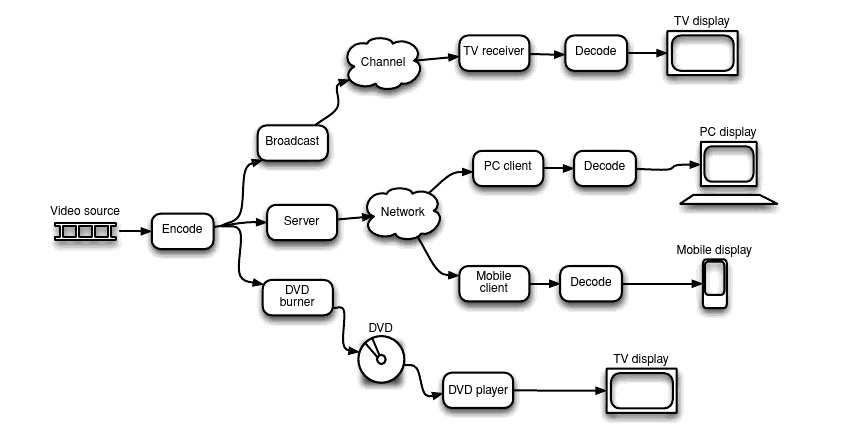
\includegraphics[width=0.8\textwidth]{codec.jpg}
	\caption{Videokoodaus mahdollistaa datan liikkuvuuden}
	\label{fig:codec}
\end{figure}

Koodauksen kolmas muoto, transkoodaus, tulisi tehdä, jos haluttu näyttölaite ei
tuekaan sille tarjottua koodaustapaa.

\subsection{Kuvadatan laadun mittarit}

Videodatan laatua voidaan mitata subjektiivisesti ja objektiivisesti.
subjektiivinen mittaaminen on vaikeaa, sillä ihmisten arvioihin vaikuttavat
monet seikat. Objektiivinen mittaaminen taas antaa selviä lukuja vastaukseksi,
mutta tulosten merkitys ja vaikutus katsojakokemukseen on selvitettävä erikseen.
Videodatan kohdalla subjektiivista mittaamista voidaan usein pitää tärkeämpänä
kuin objektiivista, sillä tavoitteena usein on mahdollisimman miellyttävän
katselukokemuksen tuottaminen käyttäjälle. (\citealt{h264}) Toisaalta videodatan objektiivinen
laatu on erityistapauksissa myös tärkeää, esimerkiksi konenäköä hyödyntävissä
sovelluksissa tai koneiden muuten tulkitessa videodataa. Videodatan määrän
kasvaessa jatkuvasti ja konenäkösovellusten, kuten robottien, lisääntyessä
saattaa objektiivisesta laadusta tulla subjektiivista tärkeämpää. (\citealt{youtube},
\citealt{cisco}).

Seuraavassa esitellään muutamia objektiivisia tapoja mitata videodatan laatua.
Subjektiivinen mittaaminen perustuu lähinnä ihmisillä tehtyihin
kyselytutkimuksiin, joilla on omat ongelmansa. Tässä työssä niihin ei keskitytä
syvemmin.

Tiheys, jolla ruutuja tallennetaan, määrää ruutunopeuden (frame rate).
Ruutunopeus ja kuvapisteiden määrä tarjoaa helpon mittarin kuvan laadulle.
Normaalitarkkuuksinen ja korkeatarkkuuksinen (Standard Definition, High
Definition) videodata eroavat toisistaan juuri kuvapisteiden määrän ja
ruutunopeuden perusteella. Valittu ruutujen tai kenttien esitystapa vaikuttaa
kuitenkin subjektiiviseen laatuun, joten ruutunopeuden ja kuvapisteiden määrää
ei voi pitää ehdottomana laadun mittarina. (\citealt{h264}, \citealt{du})

Yleisesti käytetty mittari videodatan laadun mittaamiseen on PSNR-arvo (Peak
Signal to Noise Ratio). PSNR kertoo erosta alkuperäisen ja uuden kuvan välillä
ja se on määritelty

\begin{center}
\begin{equation}PSNR_{dB} = 10\log_{10}\frac{(2^n - 1)^2}{MSE},\end{equation}
\end{center}

missä MSE on keskimääräinen neliöity virhe (Mean Squared Error) alkuperäisen 
kuvan ja uuden kuvan välillä. (\citealt{h264})

PSNR on helppo laskea ja antaa erään objektiivisen arvion videon laadusta.
Menetelmällä on puutteensa, kuten se, että alkuperäistä kuvaa ei ole
välttämättä saatavilla. Toisaalta, kuten monissa objektiivissa mittareissa,
pelkkä PSNR arvo ei vastaa suoraan mitään subjektiivista arvoa. Yleisesti
ottaen korkea PSNR arvo tarkoittaa hyvää laatua ja matala arvo huonoa.
(\citealt{h264}, \citealt{du})

\newpage

\section{Rinnakkaislaskenta}

Tässä luvussa käsitellään rinnakkaislaskennan perusteita, haasteita ja
RVC-CAL-standardi, jonka tavoite on helpottaa rinnakkaisten
videokoodausmenetelmien suunnittelua. Tekstissä esitellään lyhyesti
myös kuuluisa Amdahlin laki sekä muutama tutkimus automaattisten
rinnakkaistamisen toteutukseen.

\subsection{Erilaisia rinnakkaisuuksia}

Rinnakkaisuutta on nykypäivän tietokonejärjestelmissä monella tasolla.
Nykyaikaisissa supertietokoneissa on jopa yli miljoona ydintä (\citealt{top500}),
tavallisia tietokoneita kerätään laskentaklustereiksi, tieteellisessä
laskennassa hyödynnetään monenlaisia rinnakkaisia laskentamenetelmiä ja jopa
Internetiä voidaan pitää eräänlaisena rinnakkaislaskennan alustana. Toisaalta
suurten supertietokoneiden lisäksi rinnakkaisuus on tullut aivan tavallisten
kuluttajatietokoneiden osaksi. Prosessorit ovat jo pitkään hyödyntäneet
erilaisten laskentayksiköiden samanaikaista käyttöä laskentaa tehostaakseen.
Viimeksi mainittu menetelmä tunnetaan termillä liukuhihnaus (pipelining).
(\citealt{intro}, \citealt{rauber})

Yhteisiä eri tason rinnakkaisille ratkaisulle ovat niin hyödyt kuin haitatkin.
Kaikki tavoittelevat lisäystä suorituskykyyn, mutta rinnakkaisuuden
hallinta tuo laskentaan omia haasteitaan. Esimerkiksi liukuhihnaamisen hyödyt
käyvät ilmi seuraavasta esimerkistä. Oletetaan, että tehdas tuottaa autoja.
Kunkin auton valmistaminen kestää sata tuntia, joten valmistamalla yksi auto
kerrallaan saadaan sadassa tunnissa yksi auto. Jos auton valmistus kuitenkin
pilkotaan kymmeneen osaan, joita voi suorittaa rinnakkaisesti, ja joiden
suoritus kestää kymmenen tuntia, voidaankin sadassa tunnissa tuottaa kymmenen
autoa. Saavutettu hyöty triviaalissa esimerkissä on kymmenkertainen.
(\citealt{intro}). Toisaalta samaa esimerkkiä voidaan hyödyntää ilmentämään
liukuhihnaamisen vaikeuksia. Jos esimerkiksi kaksi peräkkäistä tehtävää
olisivat auton ovien kiinnittäminen ja maalaaminen, niin on selvää, että autoa
ei voi maalata ennen ovien kiinnittämistä. Esimerkiksi tällaiset
riippuvuussuhteet aiheuttavat ongelmia rinnakkaislaskennalle ja niitä sekä
muita haasteita varten täytyy kehittää hallintarakenteita.

Hallintarakenteita erilaisille rinnakkaisuuden muodoille on monia.
Yksinekertaiseen liukuhihnaamiseen eräs ratkaisu on suoritettavien operaatioiden
järjestäminen sellaiseen järjestykseen, että riippuvuussuhteet eivät
aiheuta ongelmia. Toisaalta liukuhihnaa voidaan myös hidastaa, jolloin
saavutettu laskentateho vähenee, mutta laskenta pysyy oikeana. Nämä
ratkaisut kuulostavat yksinkertaisilta, mutta niiden toteutukseen ja
vaikutuksiin liittyy kuitenkin haasteita, joihin ei kuitenkaan tässä työssä
syvennytä tarkemmin. (\citealt{intro}, \citealt{rauber})

Kun laskentayksiköitä on enemmän, tarvitaan monimutkaisempia
hallintamekanismeja. Huomattavaa on kuitenkin, että usein rinnakkaisuutta on
laskentayksikössä monella tasolla - esimerkiksi prosessoreita on monta, ja
jokaisella prosessorilla on oma liukuhihnansa. Monimutkaisemmat
hallintarakenteet voidaan jakaa karkeasti kahteen luokkaan sen perusteella,
miten paljon laskennan hallintaa kullekin laskentayksikölle on jaettu. Jos
hallinta on keskitetty, kyseessä on SIMD-arkkitehtuuri (Single Instruction
stream, Multiple Data stream). SIMD-arkkitehtuurissa yksittäinen
hallintayksikkö päättää, mitä kukin laskentayksikkö laskee.
MIMD-arkkitehtuurissa (Multiple Instrucrion stream, Multiple Data stream)
jokaisella laskentayksiköllä on oma hallintayksikkönsä. Konkreettisena
esimerkkinä arkkitehtuurien erona voi pitää esimerkiksi sitä, että
MIMD-arkkitehtuurissa jokainen laskentayksikkö voi suorittaa eri ohjelmia, kun
SIMD-arkkitehtuurissa hallintayksikkö päättää, mitä ohjelmaa kaikki
laskentayksiköt suorittavat. (\citealt{intro}, \citealt{rauber})

\subsection{Rinnakkaisuuden peruskäsitteitä}

Erilaisten rinnakkaisuuden muotojen lisäksi rinnakkaislaskenta voidaan jakaa
kahteen tyyppiin sen perusteella, mihin rinnakkaisuus kohdistuu.
Tehtävärinnakkaisessa laskennassa rinnakkain suoritetaan erilaisia
tehtäviä - esimerkiksi saman ohjelman eri säikeitä. Datarinnakkaisessa
ohjelmoinnissa taas rinnakkaisuus syntyy siitä, että operoidaan samaan aikaan
eri datan osa-alueilla. (\citealt{intro}) Datarinnakkainen lähestymistapa sopii hyvin
joidenkin videokoodauksen osien rinnakkaistamiseen. Esimerkiksi diskreettiä
kosinimuunnosta tehdessä, voidaan kukin lohko käsitellä erikseen, sillä ne ovat riippumattomia 
toisistaan. Saavutetut hyödyt laskenta-ajassa ovat huomattavat. Toisaalta
videodatan vahvojen riippuvuussuhteiden takia rinnakkaisuuden soveltaminen
muissa tarkoituksissa vaatii kekseliäisyyttä.

\subsubsection{Tiedon välittäminen laskentayksiköiden välillä}

Rinnakkaisuuden kohteen lisäksi rinnakkaisilla kohteilla on erilaisia tapoja
järjestää tiedon liikkuminen laskentayksiköiden välillä. Pääparadigmoja on
kaksi, jaettu muisti (shared memory) ja viestinvälitys (Message Passing Interface, MPI). Jaetun muistin mallissa
laskentayksiköillä on yhteinen muisti, josta jokainen saa lukea ja kirjoittaa.
Jotta yhteinen muisti pysyy puhtaana eli kaksi laskentayksikköä ei lue ja/tai
kirjoita samaan muistiosoitteeseen samaan aikaan, täytyy järjestelmällä
olla keinot päättää milloin mitäkin muistialuetta saa käsitellä.
Erilaisia ratkaisuja tähän ongelmaan (mutual exclusion) on useita, kuten
monitorit tai semaforit. Samojen muistialueiden käsittelyyn
liittyy myös käsite kisatilanteista (race condition). Kisatilanteessa kaksi
laskentayksikköä tavoittelee samaa muistialuetta, mutta valitun
muistinsuojausmenetelmän pitäisi estää tämä. Kisatilanteet eivät varsinaisesti
ole rinnakkaisten ohjelmien vikoja vaan syntyvät rinnakkaisohjelmoinnin
sivutuotteena. (\citealt{ari})

Viestinvälitysmenetelmän nimi kuvaa sitä hyvin. Jokaisella
laskentayksiköllä on oma muistiavaruutensa, ja jos esimerkiksi  yksiköiden
välillä halutaan synkronoida, niin ne vaihtavat viestejä. Menetelmä vaatii,
että jokaisella laskentayksiköllä on tunniste, jolla sen voi erottaa muista.
Tämä vaatimus ei koske jaetun muistin menetelmää. Luonnollisesti viestien
välittämiseen tarvitaan myös jokin kanava niiden toimittamiseen. Viestien
välittäminen on jaetun muistin käyttämistä tehottomampaa, mutta sitä
käyttämällä on helpompi pitää yllä erilaisia laskentayksiköitä. Kaikkien
käyttäessä samaa muistia yksiköiden tulee käsitellä muistia samalla tavalla,
mutta viestejä välittäessä jokaisen yksikön täytyy vain täyttä
viestinvälitysrajapinnan vaatimukset. (\citealt{intro}, \citealt{rauber})

\subsubsection{Rakeisuus ja laskennan järjestäminen}

Jotta laskentatehtäviä voidaan suorittaa rinnakkaisesti, täytyy tehtävät
hajottaa (decompose) pienempiin osiin. Hajotusta tehdessä otetaan huomioon laskennan
erilaiset riippuvuudet ja jaetaan laskentatehtävä pienempiin osatehtäviin.
Tiedot riippuvuuksista täytyy tallentaa myöhempää käsittelyä varten.
Kaikki osatehtävät eivät välttämättä ole samankokoisia ja kun jako on tehty,
kukin osatehtävä on uusi, jakamaton laskennan kohde. Tyypillisesti ohjelmoijan
tehtäväksi jää jakaa laskentatehtävät osatehtäviksi. (\citealt{intro})
Tehtävienjako voidaan tehdä myös staattisesti eli ennen ohjelman ajon
aloittamista tai dynaamisesti eli ajonaikaisesti (\citealt{rauber}).
Automatisoitua rinnakkaistamista kuitenkin tutkitaan. Erään tutkimuksen
tuloksena on laskenta-arkkitehtuuri joka optimoi peräkkäisestä koodista
rinnakkaisesti ajettavaa koodia (\citealt{apopei}). Toinen tutkimus esittää
työkalun, joka erottaa rinnakkaisuuden löytämisen ja optimoinnin sekä esittää
ohjelmointirajapinnan (API) tämän toteuttamaan (\citealt{dope}).

Osatehtävien kokoa ja määrää kutsutaan rakeisuudeksi. Jos osatehtäviä on vähän
ja ne ovat suuria, puhutaan karkeasta rakeisuudesta (coarse-grained
decomposition), kun taas suurta määrä pieniä osatehtäviä kutsutaan
hienojakoiseksi (fine-grained decomposition). Myöhemmin esitetään joitakin
rinnakkaislaskennan tehokkuuden mittareita, mutta eräs rinnakkaisuuden
tunnusluku on rakeisuuteen liittyä rinnakkaisuusaste. Korkein 
rinnakkaisuusaste kuvaa, kuinka montaa osatehtävää laskea samanaikaisesti
ohjelman ajon aikana. Korkein rinnakkaisuusaste on yleensä osatehtävien määrää
pienempi osatehtävien riippuvuussuhteiden johdosta. Korkeinta
rinnakkaisuusastetta yleisemmin käytetty rinnakkaisuuden tunnusluku on
keskimääräinen rinnakkaisuusaste, joka kertoo, kuinka monta osatehtävää oli
laskennassa keskimäärin ohjelman ajon aikana. (\citealt{intro}, \citealt{rauber})

Kun jako osatehtäviin on tehty, täytyy osatehtävä jakaa laskentayksiköille.
Purkuvaiheessa tallennetut riippuvuustiedot ovat tärkeitä laskentaa
järjestettäessä. Tässä työssä ei tarkemmin syvennytä erilaisiin
hajotustekniikoihin tai laskennan järjestämiseen, mutta muutamia
yleisperiaatteita käydään seuraavassa läpi. Tästälähin laskennan järjestämistä
kutsutaan kuvaukseksi, jonka lähtöjoukkona on looginen laskentaongelma ja kohdejoukkona fyysiset laskentayksiköt.
Hyvät kuvausalgoritmit pyrkivät hyödyntämään suuren määrän laskentayksiköitä
mahdollisimman tehokkaasti - muista riippumattomat osatehtävät eri
laskentayksiköille, mahdollisimman moni laskentayksikkö käytössä,
paljon viestivät osatehtävät samoille laskentayksiköille.
Toisaalta pitäisi pitää laskentayksiköitä vapaana sellaisille tehtäville,
joista muut tehtävät ovat riippuvaisia. Päämäärät ovat ristiriitaisia, sillä
ei ole esimerkiksi joidenkin laskentayksiköiden vapaana pitämien on selvästi
ristiriitaista mahdollisimman suuren käyttöasteen saavuttamiseksi. Sopivan
tasapainon ja hyvän kuvauksen löytäminen ei ole helppo tehtävä, ja vaikka
rinnakkaisuusaste antaa teoreettisen parhaan arvon rinnakkaisuudelle,
käytännössä kuvaus määrää, kuinka rinnakkaista laskenta oikeasti on.
(\citealt{intro}, \citealt{rauber})

\subsubsection{Amdahlin laki}

Useasti on mainittu, että rinnakkaislaskennan tavoite on laskentatehon
lisäys. Rinnakkaislaskennan laskentatehon lisäystä verrattuna peräkkäiseen
laskentaan kuvaa Amdahlin laki, joka kuuluu

\begin{center}
\begin{equation}\frac{1}{r_s + \frac{r_p}{n}},\end{equation}
\end{center}

missä $r_s + r_p = 1$ ja $r_s$ kuva ei-rinnakkaistuvaa osaa ohjelmasta,
$r_p$ rinnakkaistuvaa osaa ja $n$ laskentayksiköitä (\citealt{amdahl}).
Kaavasta voidaan päätellä, että laskentayksiköiden määrää suurentaessa
laskentateho ei kasva äärettömyyksiin.

\subsection{Rinnakkaisuuden haasteita}

Rinnakkaistaminen tehostaa laskentaa, mutta rinnakkaistaminen tuo
uudenlaisia haasteita tietokonejärjestelmien suunniteluun. Mainitut
hallintarakenteet tuovat ylimääräisiä kustannuksia laskennan oheen,
kuten viestintään liittyviä vaatimuksia.
Tietokoneiden tehokkuutta ei määrittele ainoastaan prosessorin tai
prosessorien nopeus, vaan esimerkiksi muistin vasteaika ja kaistanleveys
asettaa rajoja sille, kuinka paljon laskentaa voidaan suorittaa. Muistin
hitautta voidaan kompensoida monilla keinoilla, kuten välimuisteilla (cache),
monisäikeisyydellä (multithreading) tai ennakkohauilla (prefetching). Muistin
hitaus ei ole yksinomaan rinnakkaislaskennan ongelma, mutta ongelma pahenee
hallintakustannuksien ja monien laskentayksiköiden ongelmien kertautuessa.
(\citealt{intro})

Puhtaasti rinnakkaisuuteen liittyviä ongelmia ovat esimerkiksi tyhjäkäynti
(idling) ja turha laskeminen (excess computation). Tyhjäkäynnissä jotkin
laskentayksiköt eivät suorita mitään laskentaa. Tämä saattaa johtua esimerkiksi
siitä, että hallintajärjestelmä ei ole antanut laskentayksikölle laskettavaa,
koska tarpeeksi tehtäviä ei ole. Videokoodauksen yhteydessä mainitut
riippuvuudet aiheuttavat myös tyhjäkäyntiä. Tällöin resursseja hukataan. Turhaa
laskentaa on esimerkiksi se, että useampi laskentayksikkö laskee samaa asiaa
tahoillaan. Tällainen tilanne saattaa syntyä esimerkiksi silloin, kun
rinnakkaislaskentaan valittu algoritmi ei ole tehtävään optimaalinen. Tilanne
ei ole harvinainen, sillä monet tehokkaat peräkkäiset algoritmit käyttävät
aiemmin laskettua tietoa hyväkseen. Laskennan ollessa hajautettuna eri
laskentayksiköille aiemmin lasketun tiedon hyödyntäminen on mahdotonta.
(\citealt{intro})

\subsection{Rinnakkaisten järjestelmien tehokkuuden mittaaminen}

Aiemmin mainittiin Amdahlin laki, joka antaa karkean arvion ohjelman
rinnakkaistamisen tuomasta laskentatehon nopeuden kasvusta. Tämä ei kuitenkaan
ole ainoa tapa mitata rinnakkaisia järjestelmiä. Muita tässä käsiteltäviä tapoja
ovat rinnakkaisuuden lisäkustannukset, ohjelman suoritusaika, laskennan
tehokkuus, ja laskennan hinta. Kaikkia tuloksia voidaan verrata peräkkäisen
ohjelman vastaaviin suorituksiin ja todeta, onko rinnakkaistaminen järkevää.
(\citealt{intro})

Peräkkäisen ohjelman tapauksessa ohjelman suoritusaika on aika ohjelman
suorituksen alkamisesta sen päättymiseen, jatkossa $T_p$. Rinnakkaisen
ohjelman suoritusaika on aika rinnakkaisen ohjelman suorituksen alkamisesta
viimeisen laskentayksikön laskennan loppumiseen, jatkossa $T_r$. (\citealt{intro})

Rinnakkaisuuden lisäkustannukset muodostuvat hallintajärjestelmän kuluista,
viestien välittämisestä, synkronoinnista ja vastaavista toimista, jotka ovat
välttämättömiä rinnakkaisen laskennan onnistumiseksi. Kuvatkoon $p$
rinnakkaisen järjestelmän laskentayksiköitä, $T_p$ yhden laskentayksikön
suorittamaa laskentaa. Koko laskentaan suoritettu aika on siis $pT_p$. Olkoon
$T_h$ aika, joka on käytetty hyödylliseen laskentaan. Lisäkustannuksiin kulunut
aika $T_l$ olkoon siis $T_l = pT_p - T_h$. (\citealt{intro})

Laskentatehon nopeuden kasvu rinnakkaisessa on erityisen kiinnostava verrattuna
vastaavaan peräkkäiseen ohjelmaan. Kuten mainittua, Amdahlin laki antaa jo
arvion laskennan nopeuden kasvusta. Tässä tapauksessa vastaava peräkkäinen ohjelma ei
välttämättä ratkaise ongelmaa samalla algoritmilla, kuin rinnakkainen ohjelma. Syy
on turhan laskemisen yhteydessä mainittu joidenkin algoritmien heikko rinnakkaistuvuus.
Yleensä vertailuun valitaan tehokkain peräkkäinen algoritmi. (\citealt{intro})
Laskentatehon nopeuden kasvun saa toki myös laskemalla suoritusaikojen erotuksen,
mutta empiirinen tulos ei yksistään riitä osoittamaan rinnakkaista tai peräkkäistä
toteutusta paremmaksi.

Ihannetilanteessa rinnakkaisen ohjelman tehokkuus olisi 100\%, eli jokainen
laskentayksikkö olisi koko ajan käytössä mahdollisimman suurella
kapasiteetilla. Käytännössä tämä tilanne ei toteudu koskaan jo pelkästään
rinnakkaisuudesta koituvien lisäkustannusten takia. Tehokkuus voidaan lausua
yksinkertaisena yhtälönä

\begin{center}
\begin{equation}\frac{S}{p},\end{equation}
\end{center}

missä $S$ on laskennan nopeuden kasvu ja $p$ laskentayksiköiden määrä. 
(\citealt{intro})

Rinnakkaislaskennan hinta määritellään rinnakkaisen ohjelman ajoajan ja
käytettyjen laskentayksiköiden tuloksi. Yksittäisen laskentayksikön hinta on
nopeimman peräkkäisen algoritmin suoritusaika. Jos rinnakkaisen algoritmin
kasvu on asymptoottisesti sama kuin yksittäisen laskentayksikön algoritmin kasvu,
rinnakkaista algoritmia sanotaan hintaoptimaaliseksi. (\citealt{intro})

Skaalaus kertoo saavutetaanko rinnakkaislaskennasta laskentayksiköiden määrään
suhteessa olevaa hyötyä, eli tehostuuko laskenta laskentayksiköitä lisäämällä.
Laskentayksiköiden lisääminen ei loputtomasti kasvata rinnakkaislaskennan
tehokkuutta. Hyvin skaalautuvan rinnakkaislaskentamallin laskenta-aika pysyy
vakiona ongelmaa ja laskentayksiköiden määrää kasvattaessa. (\citealt{rauber})

\subsection{RVC-CAL-standardi}

Rinnakkaisuuden ongelmia on käsitelty aiemmissa alaluvuissa. Tässä
alaluvussa esitellään eräs keino hyödyntää rinnakkaisuutta ja sen soveltamista
videokoodaukseen. Keino on RVC-CAL, erityisesti videokoodaukseen kehitetty
CAL-ohjelmointikielen toteutus (Cal Actor Language). CALin vahvuus on se, että
sillä on kääntäjiä monille alustoille, mukaan lukien moniydinprosessorit.
RVC-CALiin on saatavilla myös avoimen lähdekoodin toteutus (\citealt{orcc}).

CAL on korkean tason toimijakeskeinen tietovuo-ohjelmointikieli (high level
actor oriented dataflow programming language). Tietovuo-ohjelmoinnissa ohjelmat
mallinnetaan suunnattuina verkkoina, joiden solmuja kutsutaan toimijoiksi.
Toimijat kuvaavat mielivaltaisen monimutkaisia laskutoimituksia ja toimijoiden
väliset kaaret tiedon liikkumista toimijoiden välillä. Liikkuva tieto
abstrahoidaan merkeiksi (token). Toimijat toistuvasti ottavat sisääntulevista kaarista
merkkejä, suorittavat laskutoimituksensa ja tuottaa merkkejä ulospäin
meneviin kaariin. Kuvan \ref{fig:dataflow} tietovuokaaviossa on viisi toimijaa,
A, B, C, D ja E. Kunkin kaaren lähtöpuolella kerrotaan, kuinka monta merkkiä
kyseiseen kaareen tuotetaan ja päättymispuolella kuinka monta merkkiä kyseinen
toimija ottaa vastaan. (\citealt{rvc})

\begin{figure}[ht]
	\centering
	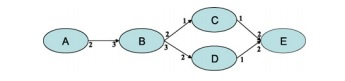
\includegraphics[width=0.5\textwidth]{dataflow.jpg}
	\caption{Yksinkertainen esimerkki tietovuokaaviosta}
	\label{fig:dataflow}
\end{figure}

Tietovuomalli perusmuodossaan ei määrää mitään aikarajoitteita toimijoiden
laskennalle. CALissa jokainen toimija on itsenäinen komponentti eivätkä muut
toimijat voi vaikuttaa sen tilaan (muuten kuin merkkejä lähettämällä). CALin
toimijat on määritelty niiden toimintojen (action) perusteella. Jokainen
toiminto määrittää miten toimijan sisäinen tila muuttuu. Toimintoja
suoritetaan (fire) riippuen merkkien sisältämästä datasta tai toimijan
sisäisistä tiedoista. Toiminnot suoritetaan peräkkäin, mutta missä toimijoiden
suoritusjärjestystä ei ole määrätty. Ominaisuuksiensa johdosta CAL sopii hyvin 
kuvaamaan rinnakkaisia järjestelmiä ja rinnakkaisia algoritmeja. (\citealt{rvc})

RVC (Reconficurable Video Coding) on MPEG-ryhmän (Moving Picture Experts
Group) kehittämä standardi rinnakkaisten videokoodausmenetelmien suunnitteluun.
Standardin tavoitteena on olla yhtenäinen, korkean tason suunnittelutyökalu.
Se määrittelee laskentayksiköt toiminnallisiksi yksiköiksi (functional unit)
ja toiminnallisten yksiköiden väliset yhteydet laskentayksiköiden välisiksi
datapoluiksi. Nämä vuorostaan kuvautuvat CALin toimijoiksi ja kuvaajien
kaariksi. CALin käyttö väliesityksenä mahdollistaa kääntämisen monenlaisille
alustoille ja jopa suoran syntetisoinnin laitteistoksi. (\citealt{rvc})

\newpage

\section{Videokoodaus ja rinnakkaislaskenta}

Tässä luvussa esitellään muutamia uusia ratkaisuja videokoodauksen
rinnakkaistamiseen. Luvun tavoite on näyttää, että vaikka rinnakkaislaskenta
tuo mukanaan suuren joukon ongelmia, niin sopivalla ongelman rajauksella
voidaan rinnakkaislaskennalla saavuttaa hyötyjä videokoodauksen saralla.

\subsection{Videokoodauksen rinnakkaistamisen tarpeellisuus}

Videokoodaus on aina ollut laskennallisesti vaativa ongelma. Viime vuosien
kehitys korkeatarkkuuksista videokuvaa kohti on johtanut siihen, että
yksiytimiset tietokoneet eivät kykene vaadittavia laskentatehtäviä suorittamaan.
Aiemmin ratkaisuna ovat olleet erilaiset multimediaan keskittyneet
laskentayksiköt, mutta niiden joustamattomuus ja hinta eivät sovellu nopeasti
kehittyvien menetelmien ja jatkuvasti kasvavien laatuvaatimusten tyydyttämiseen.
Rinnakkaisohjelmoinnin paradigma siirtää rinnakkaisuuden tietokoneen
laitteistoratkaisuista ohjelmistojen puolelle. Laitteistopohjaiset ratkaisut
ovat edelleen ohjelmistollisia ratkaisuja tehokkaampia, mutta ero pienenee
yleisluontoisten moniydinprosessorien yleistyessä ja
rinnakkaisohjelmointimenetelmien kehittyessä. (\citealt{choi})

Nykypäivänä tehokkaimmat yksiprosessorit pystyvät koodaamaan
korkeatarkkuuksista (1080p) videodataa. Kaikilla ja kaikkialla ei ole
kuitenkaan mahdollisuutta hyödyntää parhaita saatavilla olevia prosessoreita,
joten halvempia ratkaisuja on löydettävä. Samalla videodatan tarkkuus jatkaa
kasvamistaan, joten rinnakkaisuus tulee tulevaisuudessa olemaan välttämätöntä
niin multimedian esittämiselle kuin tieteellisille videokoodaussovelluksille.
On myös turha olla hyödyntämättä lisääntyvää laskentayksiköiden määrää kaikissa
tietokoneissa. (\citealt{chi}, \citealt{xu})

\subsection{Videodkoodauksen rinnakkaistamisen ongelmat}

Suurin videodatalle erityinen ongelma on jo videodataa käsitelevässä luvussa
esitellyt videodatan riippuvuudet. Joitakin ehdotuksia riippuvuuksien
karsimiseksi ehdotettiin, mutta ne eivät sovellu sellaisenaan rinnakkaisiin
ratkaisuihin. Mainittiin myös, että riippuvuuksien karsimiseen on muitakin
ratkaisuja, ja niitä käsitellään tässä luvussa. Tässä aliluvussa esitellään
tarkemmin riippuvuuksista johtuvia rinnakkaistamisongelmia sekä muita
rinnakkaislaskennan ja videokoodauksen ongelmia.

Rinnakkaisissa laskentayksiköt suorittavat laskentaa itsenäisesti, jolloin
toisten laskentayksiköiden tulostan käsiksi pääseminen on vaikeaa ja
aikaa vievää. Perinteisissä videokoodausmenetelmissä hyödynnetty ennustaminen
johtaa siihen, että sellaisenaan rinnakkaistetuissa perinteisissä menetelmissä
on paljon ylimääräisiä kustannuksia laskentayksiköiden välisestä
kommunikaatiosta ja niiden välisen synkronoinnin odottamisesta. Toisaalta
perinteisissä videokoodausmenetelmissä ruudut on jaettu lohkoihin, jotka ovat
toistaan riippumattomat. Lohkojen määrä on kuitenkin liian pieni tehokkaiden,
vahvasti rinnakkaisten ratkaisujen toteuttamiseen. Rinnakkaisuus perinteisissä
menetelmissä sellaisenaan on siis liian kallista ajan ja laskentayksiköiden
suhteen ja liian karkeaa tehokkaasti rinnakkaistuvaksi. (\citealt{pieters})

Viestinvälitysparadigmalla toimivien rinnakkaislaskentayksiköiden ongelmaksi
muodostuu viestikaistan tai kaistojen leveys. Raaka videodata, erityisesti
korkeatarkkuuksinen videodata, vaatii paljon kapasiteettia viestikanavalta. Jos
datan määrä ylittää siirtokapasiteetin, niin laskentayksiköiden käyttöaste
laskee ja rinnakkaislaskenta hidastuu merkittävästi. Luonteva ratkaisu
pullonkaulan purkamiseen olisi kanavan kapasiteetin kasvatus, mutta tämä on
useimmiten mahdotonta kustannusten, kanavan saavuttamattomuuden tai tekniikan
kehittymättömyyden johdosta. Toisinaan koodattava data on mahdollista jakaa
ennalta laskentayksiköille. Tällöin viestikanavaa ei täytetä raakadatalla ja
laskentayksiköt toimivat tehokkaasti. Reaaliaikaiseen koodaukseen tämä ei
kuitenkaan sovi. (\citealt{li})

Rinnakkainen videokoodaus kärsii siis selvästi siitä, että
videokoodausmenetelmiä ei ole alun alkaen suunniteltu rinnakkaislaskentaa
silmällä pitäen. Rinnakkaisuutta on alettu vaatia, kun laskennan vaatimukset
ovat kasvaneet, mutta standardit ja menetelmät eivät ole kehittyneet
yhtä nopeasti. Seuraavassa aliluvussa esitellään erilaisia ratkaisuja
videokoodauksen rinnakkaistamisen ongelmiin.

\subsection{Rinnakkaisia videokoodaustoteutuksia}

Rinnakkaiset videokoodausmenetelmät voidaan jakaa luokkiin esimerkiksi sen
mukaan, miten ne käsittelevät videokoodauksen rinnakkaistamisen ongelmia.
Tässä esitellyt ratkaisut perustuvat uusiin standardeihin, olemassa olevien
menetelmien riippuvuuksien ja synkronoinnin
vähentämiseen sekä olemassa olevien menetelmien optimointiin.

\subsubsection{Uudet standardit}

Rinnakkaisten ratkaisujen yleistyessä on perinteisen videokoodausmenetelmien
ongelmat alettu ottaa huomioon uusia
videokoodausstandardeja suunniteltaessa. Suunnitteilla on niin korkean
tason rinnakkaisuuden kuin matalankin tason rinnakkaisuuden poistoa. Korkean
tason rinnakkaisuus viittaa enkoodatun bittijonon rinnakkaisuuksiin ja matalan
tason rinnakkaisuus yksittäisten työkalujen ja algoritmien rinnakkaisuuksien
vähentämistä. (\citealt{choi}) Edellisessä luvussa käsitelty RVC-CAL on työkalu
rinnakkaisen videokoodauksen mahdollistamiseen ja kuuluu näin matalan tason rinnakkaisuuden
vähentämiseen.
Käsitellään seuraavaksi lyhyesti, miten kehitteillä
olevaan HEVC-standardiin (High Efficiency Vide Coding) on sisällytetty rinnakkaisuutta ja sille ehdotettua
parannusta.

HEVC-standardissa on ehdotettu joitakin keinoja rinnakkaisten
ratkaisujen pohjaksi. Ehdotettuja keinoja ovat laattapohjainen (tile based) ja
aaltorintamapohjainen rinnakkaisuus (Wavefront Parallel Processing, WPP).
Laattapohjaisessa lähestymistavassa videodatan ruudut jaetaan muuttuvan
kokoisiin laattoihin, jotka ovat toisistaan riippumattomia. Normaalista
lohkojaosta tämä poikkeaa laattojen muuttuvalla koolla, siinä missä lohkot
ovat aina saman kokoisia. Muuttuvan kokoiset lohkot mahdollistavat
samankaltaisten muotojen tai muiden kokonaisuuksien saamisen samaan laattaan,
jolloin laatan sisäinen korrelaatio on korkeampi. Ruudunlaajuiset
riippuvuussuhteet kuitenkin rikotaan ja pakkaustehokkuus laskee verrattuna
peräkkäiseen koodaukseen. Aaltorintamarinnakkaisuudessa riippuvuussuhteet
rikotaan ruutujen rivien välillä. Uuden rivin prosessointi alkaa aina edellisen
rivin toisen komponentin prosessoinnin jälkeen. Edellisen rivin toista
komponenttia käytetään seuraavan rivin ennustamiseen koodaushäviön
pienentämiseksi. Kuvassa \ref{fig:wpp} on kuvattu aaltorintamakoodauksen
eteneminen. (\citealt{chi})

\begin{figure}[ht]
	\centering
	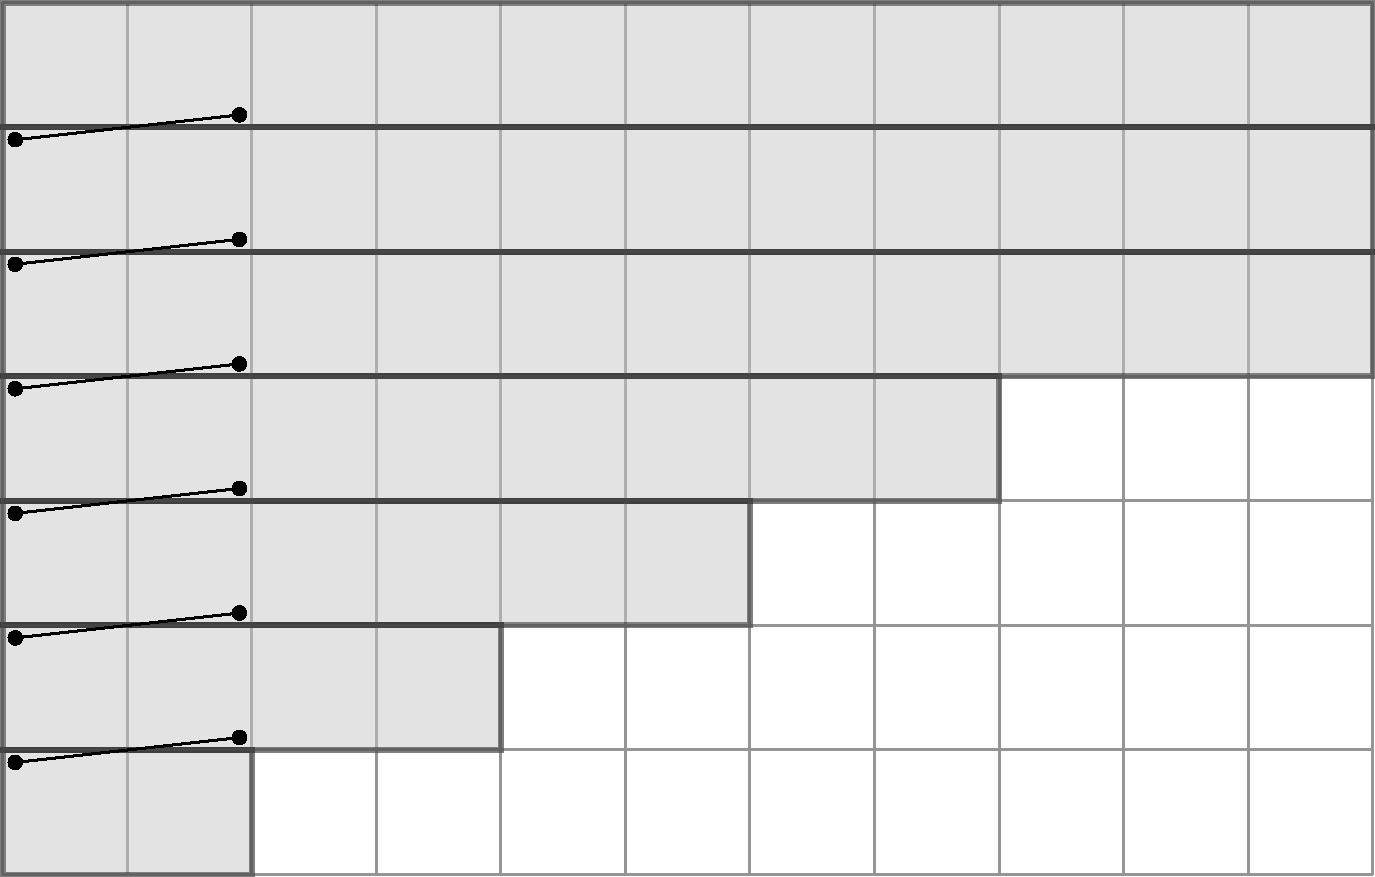
\includegraphics[width=0.5\textwidth]{WPP.jpg}
	\caption{Aaltorintamarinnakkaisen laskennan eteneminen}
	\label{fig:wpp}
\end{figure}

Aaltorintamarinnakkaisuuden riippuvuudet tarkoittavat sitä, että
laskentayksiköitä voi olla käytössä samaan aikaan ruutujen rivien verran.
Riippuvuuksista seuraa myös se, että laskentayksiköt eivät voi aloittaa
koodausta tai dekoodausta samaan aikaan, mikä aiheuttaa rinnakkaislaskennan
tehottomuutta erityisesti suurella määrällä laskentayksiköitä.
\citealt{chi} ehdottaa tähän ratkaisuksi päällekkäistä
aaltorintamaa (Overlapped Wavefront, OWF), jonka kantava idea on, että
laskentayksiköt voivat siirtyä laskemaan seuraavaa kuvaa saatuaan oman rivinsä
valmiiksi. Tämä asettaa rajoitukset sille, kuinka paljon liikekompensaatiota
voidaan käyttää. Kun komponentti tulee koodattavaksi, sen ennustamiseen
tarvittavat kompomentit täytyy olla jo koodattu. Aaltorintaman tapauksessa
tämä tarkoittaa ylempiä rivejä. Käytännössä täytyy rajoittaa ruutujenvälistä
pystysuuntaista liikekompensaatiota. (\citealt{chi})

\citealt{chi} esittää, että päällekkäinen aaltorintama tuottaa parhaat tulokset,
laattamenetelmä toiseksi parhaat ja tavallinen aaltorintama kolmanneksi parhaat
heidän testiympäristössään. Tulos antaa ymmärtää, että ehdotettu päällekkäinen
aaltorintama -menetelmä kannattaa ottaa huomioon HEVC-standardia kehittäessä.
Huomattavaa on myös, että menetelmät toimivat huomattavasti paremmin
rinnakkaisina kuin peräkkäisinä, sillä yhdessä säikeessä ajetut testit
tuottivat selvästi huonoimmat tulokset.

\subsubsection{Videodatan riippuvuuksien ja synkronoinnin tarpeen vähentäminen}

Videodatan riippuvuudet aiheuttavat sen, että rinnakakistaminen on vaikeaa tai
että suurin osa rinnakkaislaskennasta kulutetaan synkronointiin eli käytännössä
tyhjäkäyntiin. Tässä aliluvussa esitellään kaksi lähestymistapaa, joilla
riippuvuuksien määrää ja niistä seuraavia ylimääräisiä kustannuksia on pyritty
vähentämään. Edellisessä aliluvussa esitellyt aaltorintamamenetelmät ja
laattamenetelmä sopisivat tähänkin lukuun, mutta seuraavassa esitettyjä
menetelmiä ei ole ehdotettu minkään standardin osaksi.

Aaltorintamamenetelmää muistuttava rinnakkaisuutta vähentävä keino on riveittäin
suoritettava koodaus (Line-By-Line Coding, LBLC). Aaltorintaman tavoin
rivikoodaus käsittelee videodatan ruutujen rivejä. Laskentayksiköille jaetaan
kuitenkin rivien sisään rivien osia. Näin rivi koodataan rinnakkaisesti ja
koodattua riviä voidaan käyttää seuraavan rivin ennustamiseen. Rikottu
riippuvuus on siis rivien vierekkäisten osien välinen. Synkronoinnin tarvetta
on vähennetty staattisella aikataulutuksella. Saman rivin osat jaetaan eri
laskentayksiköille ja eri rivien vastaavan osat samoille laskentayksiköille.
(\citealt{xu})

Esitellyt menetelmät videokoodauksen rinnakkaistamiseen ovat keskittyneet
videodatan rinnakkaisuuden rikkomiseen. On ehdotettu myös ennustamisen
tehokkaampaa rinnakkaistamista ja näin synkronoinnin huomattavaa vähenemistä.
\citealt{pieters} esittää ennustamiseen tehokkaasti rinnakkaistuvan
rekursiiviseen kaksinkertaistamiseen (recursive doubling) perustuvaa
etuliitesummaa (prefix sum) (\citealt{blelloch}). Menetelmä saa syötteekseen
perusennustuksen sekä jäännösarvot, joiden avulla näytteiden arvot on
tallennettu, kuten normaalissakin ennustamisessa. Etuliitesumma lasketaan
rinnakkaisilla laskentayksiköillä, eikä edellisten näytteiden koodausta
tarvitse odottaa. Etuliitesumma etenee puumaisesti, minkä johdosta siinä on
korkeintaan logaritminen määrä synkronointipisteitä näytteiden määrään nähden.
Kuva \ref{fig:prefix_sum} esittelee etuliitesumman etenemisen. Puun tasot ovat
mahdollisia synkronointipisteitä. (\citealt{pieters})

\begin{figure}[ht]
	\centering
	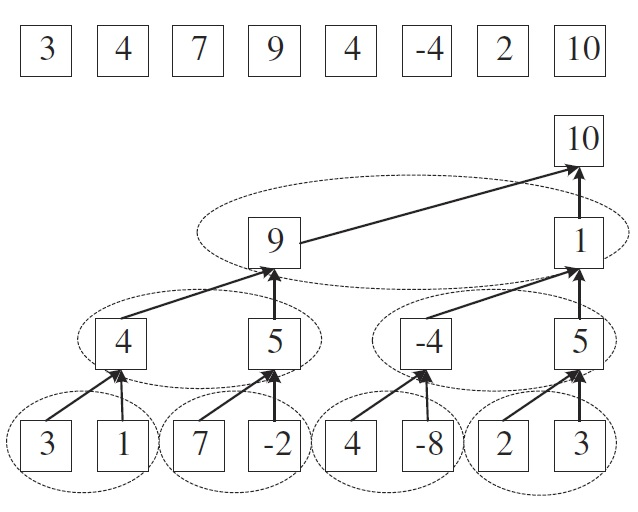
\includegraphics[width=0.5\textwidth]{prefix_sum.jpg}
	\caption{Etuliitesumma johtaa näytteen arvot jäännösarvoista}
	\label{fig:prefix_sum}
\end{figure}

Molemmat tässä kappaleessa esitellyt videokoodauksen rinnakkaistamismetodit
ovat osoittautuneet testeissä tehokkaiksi. Rivikoodaus nopeuttaa videokoodausta
lähes lineaarisesti laskentayksiköiden määrään nähden. Parhaiten se toimii
häviöttömillä ja lähes häviöttömillä koodausmenetelmillä, mikä on sopivaa,
sillä sellaiset menetelmät tarvitsevat tehokkuutta ollakseen käytännöllisiä.
(\citealt{xu}) Paremmin rinnakkaistuvat ennustaminen nopeutti H.264-standardilla
enkoodatun videon dekoodaamista 2.2-7.9 kertaisesti aaltorintamamenetelmään
verrattuna sekä 2.2 kertaista nopeutusta normaaliin ennustamiseen 2160p
-tarkkuuksisella videolla. (\citealt{pieters})

\subsubsection{Optimointi}

Uusien menetelmien kehittämisen lisäksi voidaan rinnakkaisuutta tuoda
olemassa oleviin menetelmiin niitä muuttamatta. Tällöin on tärkeää löytää
kulloinkin ratkaistavissa olevaan ongelmaan sopiva rinnakkainen lähestymistapa.
Aiemmin esiteltyjä teorioita rinnakkaisuuden mittaamisesta voidaan käyttää
erilaisten ratkaisujen analysointiin, mutta todelliset tulokset saadaan
vasta käytännön testeillä. (\cite{li})

\citealt{li} on tutkinut H.264-standardin mukaisen videokoodauksen optimointia
rinnakkaiseen järjestelmään. Tutkimus ei esitä uusia algoritmeja
videokoodauksen ongelmien ratkaisemiseen vaan tutkii erilaisia
rinnakkaislaskentaan vaikuttavia parametreja, kuten laskentayksiköiden määrää
ja konekielisen tason optimoinnin hyödyntämistä. Suurin haitta
rinnakkaislaskennan tehokkuudelle tutkimuksessa oli laskentayksiköiden välisen
viestinnän hitaus. (\citealt{li})

Tutkimuksen tulokset osoittavat, että eräänlainen raaka rinnakkaistaminen
tehostaa videokoodausta hieman. Koska H.264 ei ole suunniteltu rinnakkaiseksi,
sen rinnakkainen tehonlisäys ei kasva lineaarisesti laskentayksiköiden määrää
kasvattaessa. Samoin yksittäisen laskentayksikön tehokkuus laskee huomattavasi
laskentayksiköiden määrää lisätessä erityisesti hitaammilla
tietoliikenneyhteyksillä. Paras tulos saavutettiin esijakamalla koodattava
videodata laskentayksiköille, jolloin sen siirtämien ei enää aiheuttanut
pullonkaulaa. (\citealt{li})

\subsubsection{Rinnakkaislaskennan tuomat hyödyt suorituskykyyn}

Videodataa esittelevässä luvussa esiteltiin erilaisia mittareita videodatan
laadulle. Videokoodauksen tehokkuutta voidaan mitata esimerkiksi ruutujen
koodausnopeudella ($\frac{ruutua}{sekunti}$) tai pakkaussuhteella, eli kuinka
pieneksi data pakataan verrattuna alkuperäiseen. Alle on kerätty taulukkoon
erilaisten rinnakkaisten videokoodausmenetelmien tuomia hyötyjä
videokoodaukseen.

\begin{center}
\begin{tabular}{| p{\linewidth/4} | p{\linewidth/4}| p{\linewidth/4}| p{\linewidth/4}|}
	\hline
	Menetelmä & Mitattu suure & Saavutettu hyöty & Lähde \\
	\hline\hline
	Optimointi & Koodausnopeus & Viestikapasiteetin riittäessä lineaarinen laskentatehon kasvu laskentayksiköihin nähden
			\citealt{li}& \\
	\hline
	Rinnakkainen ennustaminen & Dekoodausnopeus &
			18.3-21.5 kertainen nopeus verrattuna aaltorintamarinnakkaisuuteen & \citealt{pieters} \\
	\hline
	Rinnakkaisuuksien rikkominen & Pakkaussuhde & Parhaimmillaan 14\% parempi pakkaussuhde verrattuna
			peräkkäiseen implementaatioon & \citealt{xu} \\
	\hline
	Rinnakkaisuuksien rikkominen & Skaalautuvuus & Lähes lineaarinen skaalautuvuus laskentayksiköiden määrään nähden &
			\citealt{xu} \\
	\hline
	Rinnakkaisuuksien rikkominen & PSNR & Korkeampi PSNR kuin peräkkäisellä menetelmällä erityisesti korkealaatuisessa videossa
			\citealt{xu}& \\
	\hline
\end{tabular}
\end{center}

\subsection{Erilaiset kiihdytysalustat}

Yksi rinnakkaislaskennan haasteista on siinä, että rinnakkaiset laskentayksiköt
ovat hyvin erilaisia ja yhteisiä tekniikoita ja toteutuksia niille on vaikea
löytää. Tässä aliluvussa käsitellään muutamia erilaisia kiihdytysalustoja ja
niiden sopivuutta rinnakkaiseen videokoodaukseen.

\subsubsection{Moniydinprosessorit}

Kaikenlaiset tietokoneet aina älypuhelimista tehokkaisiin palvelimiin alkavat
olla nykypäivänä moniydinprosessoreilla varustettuja (\citealt{choi}). Tämän
johdosta tätä kiihdytysalustaa voidaankin pitää tärkeänä erityisesti
multimediasovelluksille, joissa videokoodaus on yleinen ja tärkeä operaatio.
Esitellyistä tutkimuksista \citealt{chi} käytti kiihdytysalustanaan 12-ytimistä
prosessoria, kun taas \citealt{li} käytti klusteria moniytimisiä prosessoreita.
Esitetyt tulokset osoittavat, että videokoodaus voidaan onnistuneesti
rinnakkaistaa moniydinprosessoreille, mikä ennustaa hyvää tulevaisuuden
rinnakkaisille videokoodaustoteutuksille kuluttajatason tietokoneissa.

\subsubsection{Klusterit}

Klusteri tarkoittaa useampaa yhteen liitettyä tietokonetta, jotka on valjastettu
suorittamaan samaa tehtävää. Klusterit ovat tyypillisiä tieteelliselle ja
todella vaativalle laskennalle, joka vaatii yksittäisiä koneita suuremman 
laskentatehon. Esitellyistä tutkimuksista \citealt{li} esitteli kaksi erilaista
klusteria, toisen Windows-käyttöjärjestelmän PC:illä ja toisen
Linux-käyttöjärjestelmällä toimivilla koneilla. Klusterit tuovat 
rinnakkaislaskentaan omat haasteensa, kuten klusterin laskentayksiköiden
heterogeenisyyden, laskentayksiköiden välisen viestinnän ja esimerkiksi
klusterin hinnan. Multimedian toistamiseen klusterit ovat liian tehokkaita,
mutta esimerkiksi konenäköön tai muihin tieteellisiin sovelluksiin klustereista
ja rinnakkaisesta videokoodauksesta voi olla hyötyä.

\subsubsection{Grafiikkaprosessorit}

Grafiikkaprosessorit ovat nykypäivänä käytännössä kaikista
kuluttajatietokoneista löytyviä prosessoreita, jotka ovat erikoistuneet
grafiikan piirtämiseen näyttölaitteille. Rinnakkaiseksi kiihdytysalustaksi
grafiikkaprosessorit sopivat niiden rinnakkaisen luonteen puolesta.
Nykyaikaisissa grafiikkaprosessoreissa on satoja laskentayksiköitä, joiden
kellotaajuus ei ole suuri, mutta riittävä nopeaan rinnakkaiseen laskentaan.
Esitellyistä tutkimuksista \citealt{pieters} käytti kiihdytysalustanaan
grafiikkaprosessoria.

Grafiikkaprosessorit sopivat hyvin videokoodauksen
rinnakkaislaskenta-alustoiksi, mikä on luontevaa, piirretäänhän dekoodattu
videokuva näyttölaitteelle. Joissain uusissa näytönohjaimissa on
sisäänrakennettuna tuki ja valmiit ohjelmistoratkaisut joidenkin videokoodausstandardien dekoodaamista
varten, joten omia ratkaisuja tätä varten ei välttämättä edes tarvitse tehdä (\citealt{nvidia}).
Omille ratkaisuillekin on olemassa työkalut, esimerkiksi \citealt{pieters}
oli toteuttanut oman testiympäristönsä tunnetulla CUDA-ohjelmointikellä, joka
on kieli grafiikkaprosessoreiden ohjelmointiin.


\begin{comment}
\subsection{Muistiinpanoja}

-lähde \citealt{choi} ei ole kovin tieteellinen, mutta siinä on hyvä yleisnäkemys asiaan

-lähde \citealt{chi} kertoo yleistä tarinaa HEVC (high efficiency video coding)
menetelmien skaalautuvuudesta ja tehokkuudesta. Hyvää juttua.


-lähde \citealt{xu} ehdottaa rivi-riviltä koodausschemaa (line-by-line) monelle
ytimelle

-esittää jopa parempia tuloksia, kuin lineaarinen ratkaisu

-lähde \citealt{ut-va} käsittelee DCT:tä ja pipeliningia (helposti rinnakkaistuva
implementaatio)

-lähde \citealt{cremers} esittää koodaushinta-frameworkin, joka ottaa kantaan
videodatan liikkeeseen (motion layer decomposition) ja esittää tehokkaan
rinnakaisen algoritmin tehtävän täyttäämiseen. Paperin idea on kuvien hajotus
erilaisiin layereihin

-lähteessä \citealt{wei} enkoodataan 3D-dataa ja rinnakkaisuudella saavutetaan
varsin hyviä tuloksia

-lähteessä \citealt{lazar} on käsitelty neuroverkkoja ja enkoodausta ja dekoodausta.
Asiaa myös skaalauksesta ja GPU-klustereista

-lähteestä \citealt{pieters} löytyy datarinnakkainen näkemys massivisesti
rinnakkaisiin ympäristöihin

-lähde \citealt{li} esittelee suunnitelua ja optimointia

\end{comment}

\newpage

\section{Yhteenveto}

Tämä työ esitteli videokoodauksen ja rinnakkaisohjelmoinnin perusteita,
ongelmia ja mahdollisuuksia. Videokoodaus on tärkeää erilaisille
multimediasovelluksilla ja koneellisesti tapahtuvaan videodatan analyysiin.
Rinnakkaisohjelmointi ja -laskenta ovat kustannustehokkaita tapoja lisätä
tietokoneiden laskentatehoa ja tulevaisuudessa luultavasti ainoa tapa ratkaista
laskennallisesti vaativia ongelmia. Rinnakkaislaskentaan liittyy kuitenkin
paljon erilaisia ongelmia, joiden johdosta yhtenäisiä, tehokkaita ratkaisuja
rinnakkaislaskennan toteuttamiseksi ei ole vuosikymmenten saatossa pystytty
luomaan. Videokoodauksen haasteet taas syntyvät siitä, että videodatan määrä
ja laatu kasvavat jatkuvasti ja menetelmien on pysyttävä kehityksessä mukana.
Standardointi on kuitenkin hidasta kirjava joukko olemassa olevia standardeja
lisää haasteita erityisestä taaksepäin yhteensopivuuteen.

Videokoodauksen ja rinnakkaislaskennan yhdistäminen tarjoaa ratkaisun alati
vaativamman videodatan koodaamiseen rinnakkaislaskennan tuoman laskentatehon
kasvun myötä. Videokoodauksen rinnakakistaminen ei kuitenkaan ole ongelmatonta.
Rinnakkaislaskennan yleisten haasteiden, videodatan riippuvuuksien ja sen
vaatiman tallennus- ja siirtokapasiteetin johdosta rinnakkaislaskennan
toteuttaminen rinnakkaislaskentamenetelmillä on vaikeaa. Ongelman ratkaiseminen
on kuitenkin välttämätöntä, sillä vaikka nykypäivän tehokkaimmat yksiytimiset
prosessorit pystyvä koodaamaan korkeatarkkuuksista videota, niin tulevaisuudessa
ne tuskin siihen pystyvät eivätkä viimeistä huutoa olevat yksiytimiset
prosessorit sovellu kaikkiin videokoodausta tarvitseviin laitteisiin. Viimeisin
huuto on myös aina kalleinta, eikä se luultavimmin ole kustannustehokasta.

Kaikista vaikeuksista huolimatta rinnakkaisia videokoodaussovelluksia on tehty.
Monet niistä perustuvat videodatan rinnakkaisuuksien rikkomiseen ja täten
parempaan rinnakkaistuvuuteen, mutta pelkällä rinnakkaislaskennan tuonnilla
videokoodaukseen on saavutettu kasvua laskentatehossa Rinnakkaisten
menetelmien suorituskyky on peräkkäisiä videokoodausmenetelmiä parempi monilla
mittareilla. Tulevaisuudessa yhä enemmän videodataa käsittelevät koneet, joten
erityisesti objektiivisen laadun täytyy olla hyvä. Rinnakkaislaskennan
tehostamista kannattaa myös se, että koneet tekevät parhaat päätelmät
häviöttömästi pakatusta datasta, mikä on laskennallisesti vaativampaa.
Nykyisten ratkaisujen ongelmana on, että vaikka ne toimivat esitetyillä
testialustoilla, niiden yleistäminen esimerkiksi kaikkiin moniydinprosessorin
omaaviin kuluttajatietokoneisiin on vaikeaa.

Nyt kun rinnakkaislaskennan on osoitettu tehostavan videokoodausta, on aika
katsoa tulevaisuuteen ja miettiä, miten rinnakkaisuudet tuomat hyödyt
saataisiin kaikkien rinnakkaisten laskentayksiköiden saavutettaviksi. Tätä
tavoitetta tukevat suunnitteilla olevat uudet standardit ja menetelmät, joilla
rinnakkaisuuden alustariippuvuus vähenee ja joissa rinnakkaisuuden vaatimukset
on otettu huomioon jo suunnitteluvaiheessa. Uusimmissa näytönohjainsukupolvissa
on jo toteutettu videodatan dekoodaamisen rinnakkaisia menetelmiä.
Tulevaisuudessa tällaiset laitteistoratkaisut tulevat lisääntymään ja samalla
ohjelmistoratkaisut kehittyvät mahdollistaen rinnakkaislaskennan yleistymisen
kaikilla rinnakkaisilla laskenta-alustoilla.


% --------------------------------------------------------------------

